\section{Descrição geral do algoritmo}

O GRASP segue um ciclo multi-start (Figura~\ref{fig:pseudogeral}): em cada iteração, constrói-se uma solução viável por um procedimento guloso aleatorizado, repara-se a solução caso ela seja inviável, aplica-se a busca local e atualiza-se a melhor solução global. As iterações são independentes entre si. O critério de parada é o número máximo de iterações (100 nos experimentos finais).

\begin{figure}[H]
\centering
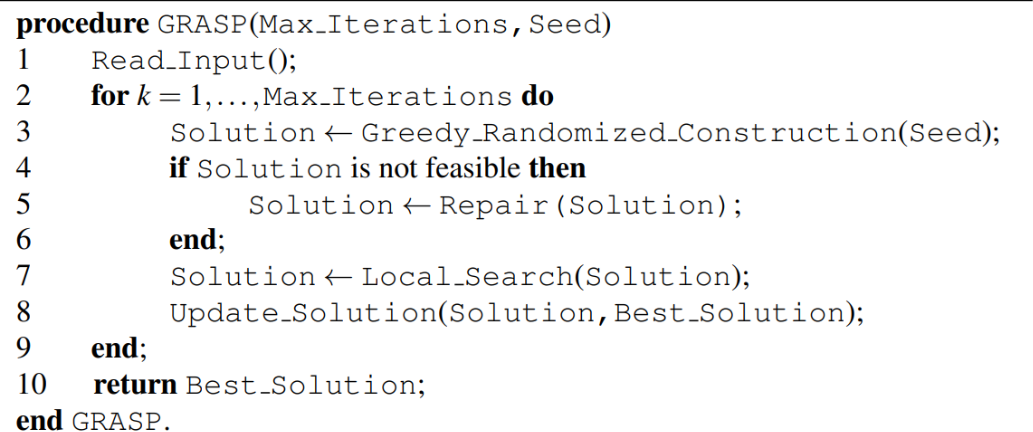
\includegraphics[width=0.50\textwidth]{imagens/pseudo-codigo-geral.png}
\caption{Pseudocódigo geral do GRASP adaptado à implementação.}
\label{fig:pseudogeral}
\end{figure}

No GRASP clássico, o parâmetro $\alpha$ da lista restrita de candidatos (RCL) permanece constante. No GRASP Reativo, $\alpha$ é sorteado a cada iteração dentre uma grade $\mathcal{A}$ de valores ($0$ a $1$, com passo $0.05$, totalizando 21 valores). Inicialmente, cada valor de $\mathcal{A}$ é usado uma vez, e o custo obtido passa a ser seu custo médio $\bar F(\alpha)$. A cada bloco de 2 iterações, $\bar F(\alpha)$ é recalculado com as soluções do bloco, e a probabilidade de escolher $\alpha$ passa a ser
\begin{equation}
p(\alpha)=
\frac{\left(F_{\mathrm{melhor}}/\bar F(\alpha)\right)^\delta}
{\displaystyle\sum_{\beta\in\mathcal{A}}
\left(F_{\mathrm{melhor}}/\bar F(\beta)\right)^\delta},
\end{equation}
em que $F_{\mathrm{melhor}}$ é o menor custo encontrado até então. A normalização faz as probabilidades somarem 1, e $\delta=5$ controla a preferência por valores de $\alpha$ com bom desempenho: quanto maior $\delta$, mais forte a preferência. O ótimo conhecido da instância não é usado nesse cálculo. No reativo, as 21 avaliações iniciais contam entre as 100 do orçamento, de modo que os dois métodos avaliam o mesmo número de soluções.

O $\alpha$ do GRASP clássico é escolhido antes dos experimentos finais, por calibração (Seção~\ref{sec:experimentos}).
